\documentclass[12pt]{article}

\usepackage[hidelinks]{hyperref}
\usepackage{comment}
\usepackage{color,graphicx,amsthm,amssymb,amsmath,cite,xspace,setspace}
\usepackage[small,bf]{caption}
\usepackage{multicol,multirow}
\usepackage{algorithm,algpseudocode}
\usepackage{soul}
\usepackage{colortbl}
\usepackage{rotating}
\usepackage{textcomp}
\usepackage{epsf}
\usepackage{wasysym}
\usepackage{mdwtab}
\usepackage{bm}
\usepackage{verbatimbox}
\usepackage{framed} % To be able to frame theorems and stuff
\usepackage{adjustbox}
\usepackage{url}
\usepackage{mathtools}

\newtheorem{theorem}{Theorem}

\PassOptionsToPackage{hyphens}{url}\usepackage{hyperref}

\usepackage[final]{pdfpages}
\usepackage{float}


% Default fixed font does not support bold face
\DeclareFixedFont{\ttb}{T1}{txtt}{bx}{n}{10} % for bold
\DeclareFixedFont{\ttm}{T1}{txtt}{m}{n}{10}  % for normal

% Custom colors
\usepackage{color}
\definecolor{deepblue}{rgb}{0,0,0.5}
\definecolor{deepred}{rgb}{0.6,0,0}
\definecolor{deepgreen}{rgb}{0,0.5,0}

\usepackage{listings}

% Python style for highlighting
\newcommand\pythonstyle{\lstset{
language=Python,
basicstyle=\ttm,
otherkeywords={self},             % Add keywords here
keywordstyle=\ttb\color{deepblue},
emph={MyClass,__init__},          % Custom highlighting
emphstyle=\ttb\color{deepred},    % Custom highlighting style
stringstyle=\color{deepgreen},
frame=tb,                         % Any extra options here
%frame=none,
showstringspaces=false            % 
}}


% Python environment
\lstnewenvironment{python}[1][]
{
\pythonstyle
\lstset{#1}
}
{}

% Python for external files
\newcommand\pythonexternal[2][]{{
\pythonstyle
\lstinputlisting[#1]{#2}}}

% Python for inline
\newcommand\pythoninline[1]{{\pythonstyle\lstinline!#1!}}

% define the type of list to use
\usepackage[shortlabels]{enumitem}
\setlist[enumerate,1]{\bfseries 1., itemsep=6mm}
\setlist[enumerate,2]{\bfseries a), itemsep=3mm}

\def\wl{\par \vspace{\baselineskip}} 
\def \bx{\boldsymbol{x}}
\def \bw{\boldsymbol{w}}
\def \bnu{\boldsymbol{\nu}}
\def \by{\boldsymbol{y}}
\def \bz{\boldsymbol{z}}
\def \bu{\boldsymbol{u}}
\def \bv{\boldsymbol{v}}
\def \bb{\boldsymbol{b}}
\def \bg{\boldsymbol{g}}
\def \ba{\boldsymbol{a}}
\def \bb{\boldsymbol{b}}
\def \be{\boldsymbol{e}}
\def \bt{\boldsymbol{t}}
\def \bd{\boldsymbol{d}}
\def \bc{\boldsymbol{c}}
\def \bA{\boldsymbol{A}}
\def\bU{\boldsymbol{U}}
\def \bB{\boldsymbol{B}}
\def \bC{\boldsymbol{C}}
\def \bX{\boldsymbol{X}}
\def \bY{\boldsymbol{Y}}
\def \bT{\boldsymbol{T}}
\def \bP{\boldsymbol{P}}
\def \bV{\boldsymbol{V}}

\def \bE{\boldsymbol{E}}
\def \bS{\boldsymbol{S}}
\def \bW{\boldsymbol{W}}
\def \bR{\boldsymbol{R}}
\def \bQ{\boldsymbol{Q}}
\def \bSigma{\boldsymbol{\Sigma}}
\def \bI{\boldsymbol{I}}
\def \bM{\boldsymbol{M}}
\newcommand{\norm}[1]{\left\|#1\right\|}

\def\R{{\mathbb R}}
\def\E{{\mathbb E}}
\def\P{{\mathbb P}}
\def \X{{\cal X}}
\def \Y{{\cal Y}}

\DeclareMathOperator{\rank}{rank}
\DeclareMathOperator{\Sign}{sign}
\DeclareMathOperator{\argmin}{argmin}
\DeclareMathOperator{\Tr}{Tr}
\DeclareMathOperator{\diag}{diag}
 

\usepackage{fullpage}

% Header and footer
\usepackage{fancyhdr,lastpage}
\pagestyle{fancy}
\rhead{}
\cfoot{\thepage\ of \pageref{LastPage}}
\renewcommand{\headrulewidth}{0.0pt}
\renewcommand{\footrulewidth}{0.0pt}


\begin{document}
\begin{center}
{\large \textbf{IRLS Algorithm in Matrix Completion}}\\
\mbox{ }\\
Enkhzaya Enkhtaivan: enkhtaivan@wisc.edu\\
Yifan Hong: yhong84@wisc.edu\\
Xiaosheng Liu: xliu878@wisc.edu\\
\mbox{ }\\
\end{center}

%
%\begin{adjustbox}{minipage=[t][.6in]{0.7\textwidth},fbox}
%Name: Enkhzaya Enkhtaivan: enkhtaivan@wisc.edu 
%
%    Yifan Hong: yhong84@wisc.edu
  
%    Xiaosheng Liu: xliu878@wisc.edu
%
%\end{adjustbox}

\begin{abstract}
As a cost-effective alternative, various low-rank matrix completion (LRMC) algorithms have been proposed over the years. In class we learned ISVT algorithm that requires the rank of original matrix. In this activity, we’ll discuss the Iteratively Reweighted Least Squares(IRLS) minimization technique that do not require the rank information. 

Since the rank minimization problem is NP-hard, it is computationally intractable when the dimension of a matrix is large. In order to avoid computational issue, we can replace the non-convex objective function with its convex surrogate. One way of doing that is shrinking all singular values equally to approximate the matrix rank, which is called nuclear norm minimization (NNM). One computationally efficient way to solve it is IRLS minimization technique. 

After completing this activity, students will be able to 1) understand the basic concept of NNM and IRLS; 2) use IRLS minimization technique to solve NNM problem; 3) understand the matrix completion problem and its application in high-level.

\end{abstract}




\section{Introduction}


Simply put, the rank minimization problem is a task to find a matrix of minimum rank satisfying a set of linear constraints e.g,:

\centerline{minimize $\rank (X)$}
\centerline{$\mathcal{L}(X) = M$}
with $\mathcal{L}$ is a linear operator encoding the linear constraints and $M$ is the observed data. In general, this problem is non-convex and has doubly-exponential running time both in theory and practice \cite{NNM}; however, when both the matrix we seek to recover and the constraints are simple enough, one can solve the problem reliably fast. One such example is the task of matrix completion, which can be applied to collaborative filtering problems such as the Netflix problem. The reason why the unknown matrix is considered to have a low rank is because an individual user's ratings is typically a combination of only a few factors such as genre, running time, inclusion of favorite actors/actresses etc.  

In this paper, we explore what is called the Nuclear Norm Minimization (NNM) -  a convex relaxation of the NP-hard problem of rank minimization. The iterative solver we employ in order to solve a NNM problem is called Iteratively Reweighted Least Squares (IRLS). Finally, we will see a demonstration of this method on a problem of Matrix Completion, which we solved in class by using Iterative Singular Value Thresholding and compare their performances. 

Here, we briefly note the advantages of using IRLS. First, this method does not require knowing the matrix of the matrix we wish to recover in contrast to ISVT. Furthermore, we solve a reweighted least squares problem at each iteration of the algorithm, which enables us to use various least squares problem solvers, such as Gauss-Newton, Gradient Descent etc.

On the other hand, the same fact that we use a least squares problem at each iteration might cause longer running time and sometimes unstability when condition numbers of the matrices involved become too high. These issues are fixed by method of stabilizing, which will be described in the section $1.2. $

\subsection{Formulation of the problem and mathematical foundation.} 

Given a matrix $\bX \in \mathbb{R}^{m \times n}$ with only partially observed data  $\Omega\subseteq\R$, we want to find its missing entries. In class, we learned about several different matrix norms such as the operator norm:
\[\begin{aligned}\|\bX\| &=\sup \left\{\|\bX \bw\|: \bw \in \R^{n} \text { with }\|\bw\|=1\right\} \\ &=\sup \left\{\frac{\|\bX \bw\|}{\|\bw\|}: \bw \in \R^{n} \text { with } \bw \neq 0\right\} \end{aligned}
    .\]
where $\|\cdot\|$ is any vector norm on $\R^n$, and the entrywise $p$- norm:
\[\|\bX\|_p =\left(\sum_{i=1}^m\sum_{j=1}^n
    |x_{ij}|^{p}\right)^{\frac{1}{p}}.\]
    
In this paper, the norm of particular interest is the Schatten $p$ - norm:
\[\|\bX\|_{S_p} = \left(\sum_{i=1}^r\sigma_i^p(\bX) \right)^{\frac 1p}\]
where $\sigma_1(\bX)\geq\sigma_2(\bX)\geq\dots \sigma_r(\bX)\geq 0 $ are the singular values of the rank $r$ matrix $\bX.$ We have seen this when $p = 2:$
\[\|\bX\|_{S_2} = \left(\sum_{i=1}^r\sigma_i^2(\bX) \right)^{\frac 12}  = \|\bX\|_F,\]
the Frobenius norm. However, our main algorithm makes use of what is called the nuclear norm:
\[\|\bX\|_*\vcentcolon =\|\bX\|_{S_1} = \sum_{i=1}^r\sigma_i(\bX).\]
A property of the nuclear norm, or the Schatten $p$ -  norm in general, that enables us to solve the NP - hard problem of rank minimization is that the $\textit{ smooth Schatten - p function}$:
\[f_p(\bX) = \left(\sum_{i=1}^r\sigma_i(\bX)^p+\gamma\right)^{\frac p2} = \Tr(\bX^T\bX+\gamma\bI)^{\frac p2},\]
is convex for $p\geq 1$ and $\gamma\geq 0 $, $[2]$. In particular, we deduce that the nuclear norm $f_1(\bX) = \|\bX\|_*$ with $p = 1$ and $\gamma = 0$ is convex. 

Finally, under suitable conditions on the matrix $\bX,$ the solution to the convex relaxation:

\begin{align}
 & \text{minimize } \|\bX\|_*\nonumber \\
 & \text{subject to } \mathcal{L}_\Omega(\bX) = \bM
\end{align}


    
\begin{align}
 & \text{minimize } \rank(\bX)\nonumber \\
 & \text{subject to } \mathcal{L}_\Omega(\bX) = \bM
\end{align}


coincide. A sufficient condition for when this happens is called the Restricted Isometry Property and we refer the readers to \cite{NNM} and \cite{IRLS- arxiv} for the rigorous details. 


\subsection{IRLS Algorithms}
In the general affine rank minimization problem, we are optimizing subject to the following constraint:

\centerline{$\mathcal{L}(\bX) = \bM$}

where $\bX\in\mathbb{R}^{m\times n},$ $\bM$ is either a matrix or a vector data and $\mathcal{L}$ is a linear operator on $\mathbb{R}^{m\times n}.$  For the special case of matrix completion problem, the linear operator is simply:
\[(\mathcal{L}_\Omega (\bX))_{ij} = \begin{cases}
\bX_{ij} \text{ if } (i,j)\in\Omega \\
0 \text{ otherwise}
\end{cases}\]
with $\Omega$ is the set of given entries of $\bX.$
 We assume that the given entries of the matrix are being sampled from some random distribution.There are several implementations and variations of the IRLS algorithm, and let us first provide simple the IRLS - M the algorithm below, as implemented in \cite{IRLS- arxiv}:

\begin{algorithm}
\caption{IRLS - M}
\begin{algorithmic}[1]
\State Input: a constant $K \geq \rank{\bX}$, a scaling paramter $\gamma > 0$
\State Initialize: $\bW_0 = \bI\in\mathbb{R}^{m\times n}$, iteration counter $k = 0$

\While{not converged}
\State $\bX_k =\underset{\mathcal{L}_\Omega(\bX)=M}{\argmin} \norm {(\bW_{k-1})^\frac 12 \bX}_F^2$
\State $\varepsilon_k = \min\left\{{\varepsilon_{k-1}, \gamma\sigma_{K+1}(\bX_k)}\right\}$
\State $[\bU_k, \bS_k^2, \bU_k^T]=\text{svd}(\bX_k\bX_k^T)$
\State $\bW_k = \bU_k(\bS_{k,\varepsilon_k})^{-1}\bU_k^T.$
\State $k = k+1;$
\EndWhile
\end{algorithmic}
\end{algorithm}
\newpage
Let us elaborate a bit on the algorithm above. Here we are solving a weighted least-squares problem at each iteration to obtain the k-th guess $\bX^k$ and subsequently the k-th weight $\bW^k.$ The appearance of the Frobenius norm is explained by following simple observation:
\[\norm{\bX}_* = \Tr[(\bX\bX^T)^{-\frac 12}(\bX\bX^T)] = \norm{\bW^{\frac 12}\bX}_F^2,\]
where $\bW = (\bX\bX^T)^{-\frac 12}$. 
The square root of a matrix is uniquely defined when the matrix is PSD (positive semi-definite)  and we indeed have a symmetric, PSD matrix since $\bX\bX^T$ is symmetric and PSD for any matrix $\bX.$ 

About the stabilization parameters $\varepsilon_k,$ the line $4$ in the algorithm ensures that it is decreasing so our algorithm does not go on indefinitely. On the other hand, we define $\bW_k$ in terms of the $\varepsilon_k$ - stabilization of $\bX_k\bX_k^T$ in order to ensure that all of our matrices used in the operations are not ill-conditioned. That is, if some of the singular values of a matrix $\bY$ are too small,  we bump up the singular values that are smaller than the threshold by doing the following:
\[\bY =\bU\bS\bV^T\implies \bY_\varepsilon = \bU\bS_{\varepsilon}\bV^T, \]
where $\bS_\varepsilon = \diag(\max\{\varepsilon, \sigma_j\})$ with $\sigma_j$'s being the singular values of $\bY$ or the entries of the diagonal matrix $\bS.$ Finally, the line $5$ uses the fact that given the Singular Value Decomposition:
\[\bY = \bU\bS\bV^T,\]
the matrix $\bY\bY^T$ has the Singular Value Decomposition:
\[\bY\bY^T = \bU\bS^2\bU^T,\]
which also coincide with its eigendecomposition. For more rigorous explanation about the algorithm and proofs of its stability and convergence, we refer the readers to \cite{IRLS- arxiv}.

\subsection{IRLS applications}

There are many applications in the matrix completion problem solved by IRLS algorithm, and here we briefly mention one of them in the field of compressed sensing. The general problem is to recover the lost entries of a signal and if the signal is sparse in some appropriate meaning of the word, then it is possible to recover the signal efficiently by sampling only a portion of the matrix. 

It was known for some time that we can do this due to what is called the Nyquist - Shannon sampling theorem \cite{sample}. However, the usage of IRLS made it clear that one can achieve even better efficiency as the theoretical was work pioneered in the work of Candes and Tao  \cite{Candes-Tao} showed. Below is a very brief example demonstrating the power of this method. 

The following 4 pictures represent a simple progress of applying NNM - IRLS to matrix.

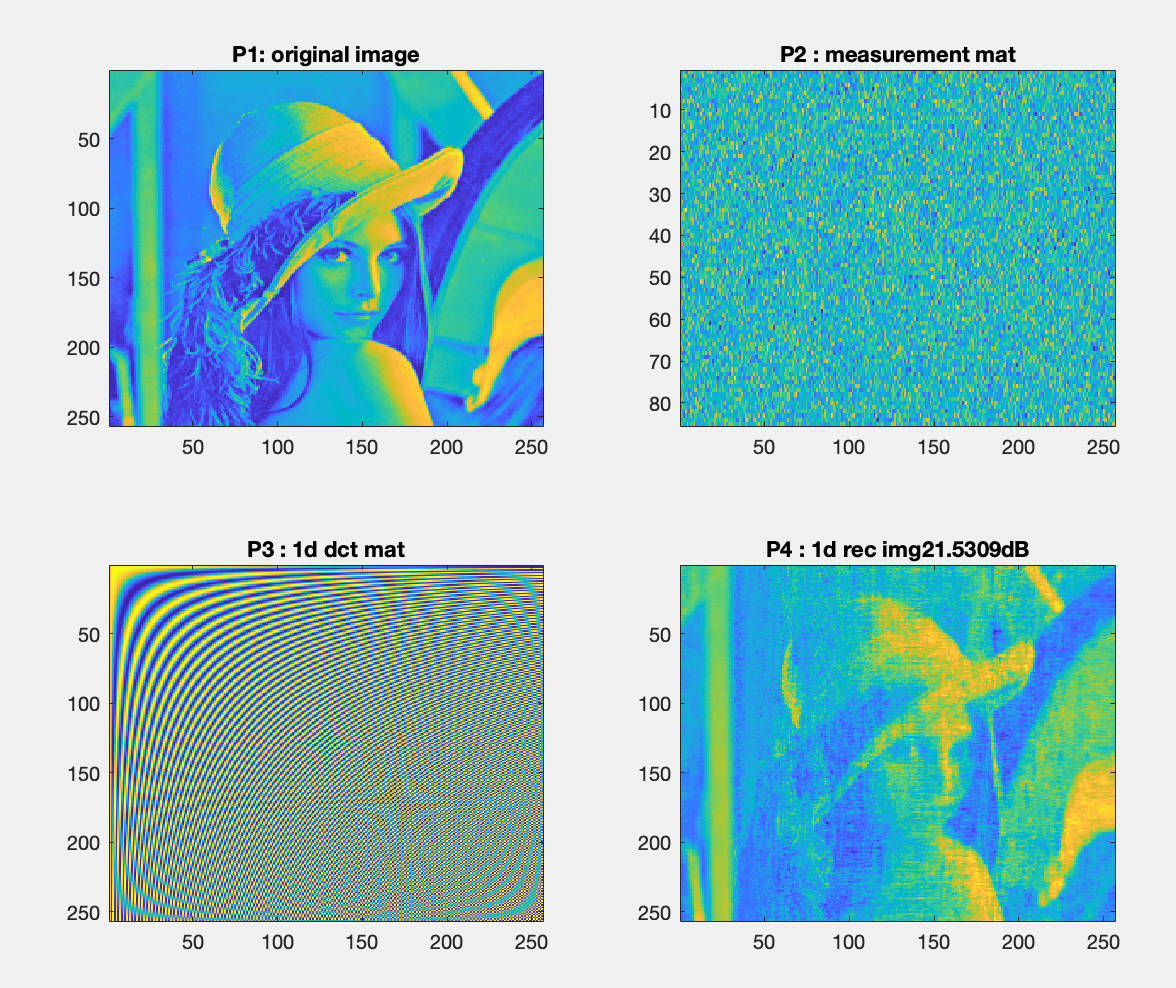
\includegraphics[width=1\textwidth]{lena1.png}

$$\min _{\bu}\|\bu\|_{1}, \quad \text { subject to } \boldsymbol{\Phi} \bu=\bb$$
Based on the formula above, P1 is the original image I with a dimension of 256*256. We randomly pick one third rows of the original image as a new matrix $\Phi$(P2) and then, reconstruct a new matrix Y = I$\Phi$. We treat each column of Y as the b in the algorithm. For every column in Y, we will use IRLS to compute a u with minimum one norm. Finally, these $u_{i}$ are put in a matrix U(P4) which is a recovery of the original image. \cite{IRLS Applications}
P3 is a very common method to make image processing more accurately and efficiently.

Roughly speaking, we are applying IRLS - NNM algorithm successively to randomly chosen rows of the given image P2 and we recover the image P4. As one can clearly see, this is a remarkable recovery considering that the given image P2 hardly looks anything like the original image. 
\section{Warm-up}
\begin{enumerate}
\item Based on the knowledge of rank minimization, which of the following is true?
    \begin{enumerate} 
        \item Rank minimization is a special case of matrix completion.

        \item When applying rank minimization, we don't limit the rank of original matrix.

        \item  Rank minimization problem can be solved in polynomial time.

        \item The missing values position in matrix $\bM$ is typically assumed to be randomly distributed. 
    \end{enumerate}

\item Which of the following is/are true?

    \begin{enumerate}

        \item Semi - definite program can solve rank minimization efficiently
        in any kinds of matrix.

        \item rank minimization problem is applied in many fields of science and technology, such as signal processing, collaborative filtering, compressed sensing.

        \item One of the advantages of IRLS over linear programming and convex programming is that it can be solved by numerical iterative solvers such as Newton - Gauss method. 

        \item Each step of the proposed algorithm requires the computation of singular value thresholding and the solution of a (usually small) least squares problem.
    \end{enumerate}
    
\item We saw that the nuclear norm is a special case of the Schatten $p$ -  norm and is convex. In addition, we used the following identity in the algorithm:
\[\|\bX\|_* = \|\bW^{\frac 12}\bX\|_F.\]
Prove the above identity by using the fact that $\bW = (\bX\bX^T)^{-1/2}$ and its square root $\bW^{\frac 12}$ is symmetric PSD and the fact that the trace function is invariant under cyclic permutations of its inputs; that is:
\[\Tr(\bX\bA) = \Tr(\bA\bX).\]
\end{enumerate}


\section{Main activity}

\begin{enumerate}
    \item \textbf{Weighted least squares(WLS)} WLS is a generalization of ordinary least squares and linear regression in which the errors covariance matrix is allowed to be different from an identity matrix. One can minimize the weighted sum of squares:\\
        $$\underset{\boldsymbol \beta}{ \operatorname{arg\,min} }\, \sum_{i=1}^{m} w_i \left|y_i - \sum_{j=1}^{n} X_{ij}\beta_j\right|^2 = \underset{\boldsymbol \beta}{ \operatorname{arg\,min} } \, \big\|W^{1/2} (\mathbf y - X \boldsymbol \beta) \big\|^2$$
    The closed form solution is similar to least square problems:\\
        $$\hat{\boldsymbol{\beta}} = (X^{\rm T} W X)^{-1} X^{\rm T} W \mathbf y$$
    
    \begin{enumerate}
    \item Consider the following matrix and vector:\\
$$ \bX = \left [ \begin{matrix} 1 & 0 \\ 1 & -1 \\ 0 & 1 \end{matrix} \right ], \boldsymbol{y} = \left [ \begin{matrix} -1 \\ 2 \\ 1 \end{matrix} \right ] $$
    Find the solution $\boldsymbol{\hat{\beta}}$ to $\underset{\boldsymbol \beta}{ \operatorname{arg\,min} } \,||\boldsymbol{y} -\bX\boldsymbol{{\beta}}||^2$
    \item Now let weight matrix $$ \boldsymbol{W} = \left [ \begin{matrix} 4 & 0 & 0 \\ 0 & 2 & 0 \\ 0 & 0 & 1 \end{matrix} \right ] $$
    Find the solution  $\boldsymbol{\hat{\beta}}$ to $\underset{\boldsymbol \beta}{ \operatorname{arg\,min} } \, \big\|W^{1/2} (\boldsymbol{y} -\bX\boldsymbol{{\beta}}) \big\|^2$
    \end{enumerate}

    \item In this section we'll use the data file \textbf{incomplete.mat} from period 15 activity, which contains a rank-2, 16-by-16 matrix $\bX_{true}$ with integer entries and three versions of this matrix ($\boldsymbol{Y_1}$, $\boldsymbol{Y_2}$ and $\boldsymbol{Y_3}$) with differing numbers of missing entries. The missing entries are indicated by NaN.\\
    Attached python script provided IRLS-M algorithm for you to perform low-rank matrix completion. The function of this algorithm requires two inputs: i) the matrix with missing entries, and ii) the upper bound of matrix rank (recall that the precise rank is unnecessary in IRLS-M algorithm).
    \begin{enumerate}
    \item Complete the missing step in function IRLS\_M. 
    \item Assuming the upper bound of rank is 3, apply IRLS-M algorithm to the three incomplete matrices. Compare your recovered completed matrices $\boldsymbol{\hat{Y_i}}$ to $\bX_{true}$ by computing the squared error $||\boldsymbol{\hat{Y_i}} - \bX_{true}||^2_F$. Does the number of missing entries affect the accuracy of the completed matrix?
    \item Now try different $\gamma$ ($ = 3, 2, 1, 0.1, 0.01 ...$) on incomplete matrix and also compute the squared error. Comment on the impact of using different $\gamma$ in the completion process.
    \end{enumerate}
    
    \item \textbf{Performance evaluation} In our script we also provided iterative singular value thresholding (ISVT) algorithm we learned in $4.6$. File \textbf{Y.txt} and \textbf{Xtrue.txt} respectively contains a rank-5, 200-by-200 incomplete matrix $\boldsymbol{Y}$ and and its complete version $\boldsymbol{Xtrue}$. Perform ISVT and IRLS-M algorithm on $\boldsymbol{M}$ with different rank parameter, compare their running time, number of iterations and accuracy. Comment on your result. (Running the python script may take several minutes. Please be patient!)\\
\end{enumerate}
\newpage

\begin{thebibliography}{9}
\bibitem{IRLS- arxiv} 
Massimo Fornasier, Holger Rauhut, and Rachel Ward. 
\textit{Low-rank matrix recovery via iteratively reweighted least squares minimization}. 
\\\texttt{https://arxiv.org/pdf/1010.2471.pdf}
 
\bibitem{IRLS rank minimization} 
Karthik Mohan and Maryam Fazel.
\textit{Iterative Reweigthed Algorithms for Matrix Rank Minimization.} 
 
Journal of Machine Learning Research 13 (2012) 3441 - 3473.
 
\bibitem{NNM}
Benjamin Recht, Maryam Fazel and Pablo A. Parrilo.
\textit{Guaranteed Minimum Rank Solutions of Matrix Equations via Nuclear Norm Minimization.} 
\\\texttt{https://people.eecs.berkeley.edu/~brecht/papers/07.rfp.lowrank.pdf}

\bibitem{IRLS Applications}
Chartrand R, Yin W. Iteratively reweighted algorithms for compressive sensing[C]//2008 IEEE International Conference on Acoustics, Speech and Signal Processing. IEEE, 2008: 3869-3872.


\bibitem{Candes-Tao}
Emmanuel Candes and Terence Tao.
\textit{The Dantiz Selector: Statistical Estimation when p is much larger than n.} 
Annals of Statistics 2007, Vol. 35, No. 6, 2313-2351.

\bibitem{sample}
\url{https://en.wikipedia.org/wiki/Nyquist%E2%80%93Shannon_sampling_theorem}
\end{thebibliography}  
\newpage
\section{Appendix}
\textbf{{\large Warm-up solution}}
\mbox{ }\\
\mbox{ }\\
\begin{enumerate}
\item d.
\item b,c.
\item
\[\|\bW^{1/2}\bX\|_F = \Tr((\bW^{1/2}\bX)^T\bW^{1/2}\bX) = \Tr(\bX\bX^T(\bW^{1/2})^T\bW^{1/2}) =\Tr(\bW\bX\bX^T) = \]
\[= \Tr\left((\bX\bX^T)^{-1/2}\bX\bX^T \right) = \|\bX\|_*.\]
\end{enumerate}

\textbf{{\large Activity solution}}
\mbox{ }\\
\mbox{ }\\


\begin{enumerate}
    \item \textbf{Weighted least squares(WLS)} WLS is a generalization of ordinary least squares and linear regression in which the errors covariance matrix is allowed to be different from an identity matrix. One can minimize the weighted sum of squares:\\
        $$\underset{\boldsymbol \beta}{ \operatorname{arg\,min} }\, \sum_{i=1}^{m} w_i \left|y_i - \sum_{j=1}^{n} X_{ij}\beta_j\right|^2 = \underset{\boldsymbol \beta}{ \operatorname{arg\,min} } \, \big\|\bW^{1/2} (\mathbf y - \bX \boldsymbol \beta) \big\|^2$$
    The closed form solution is similar to least square problems:\\
        $$\hat{\boldsymbol{\beta}} = (\bX^{\rm T} \bW \bX)^{-1} \bX^{\rm T} W \mathbf \by$$
    
    \begin{enumerate}
    \item $\boldsymbol{\hat{\beta}} = (\bX^T \bX)^{-1}\bX^T\by = \frac{1}{3}\left [ \begin{matrix} 1 \\ -1 \end{matrix} \right ]$
    \item $\boldsymbol{\hat{\beta}} = (\bX^T \bW \bX)^{-1}\bX^T \bW \by \approx \left [ \begin{matrix} -0.43 \\ -1.28 \end{matrix} \right ]$
    \end{enumerate}

    \item In this section we'll use the data file \textbf{incomplete.mat} from period 15 activity, which contains a rank-2, 16-by-16 matrix $\bX_{true}$ with integer entries and three versions of this matrix ($\boldsymbol{Y_1}$, $\boldsymbol{Y_2}$ and $\boldsymbol{Y_3}$) with differing numbers of missing entries. The missing entries are indicated by NaN.\\
    Attached python script provided IRLS-M algorithm for you to perform low-rank matrix completion. The function of this algorithm requires two inputs: i) the matrix with missing entries, and ii) the upper bound of matrix rank (recall that the precise rank is unnecessary in IRLS-M algorithm).
    \begin{enumerate}
    \item 
    \begin{python}
    W = U @ np.diag(s**(-1)) @ U.T
    \end{python}
    \item 
    $\boldsymbol{\hat{Y_1}}$ error: 12.7\\
    $\boldsymbol{\hat{Y_2}}$ error: $6.7 * 10^{-6}$\\
    $\boldsymbol{\hat{Y_3}}$ error: $3.4 * 10^{-7}$\\
    Yes, when the number of missing entries getting larger, the errors are larger. The second and third example has the relatively small number of missing entries and recovery perfectly.
    \item For $\boldsymbol{\hat{Y_1}}$:\\
    Gamma = 3 , Error: 12.6938091154\\
    Gamma = 2 , Error: 12.6938091154\\
    Gamma = 1 , Error: 12.6938091154\\
    Gamma = 0.5 , Error: 12.1753757731\\
    Gamma = 0.1 , Error: 11.8730828699\\
    Gamma = 0.01 , Error: 11.8643645163\\
    When $\gamma$ getting smaller, the error also goes down. But a smaller $\gamma$ will lead to longer running time, mostly we'll set $\gamma = 1$ in our IRLS-M algorithm.
    \end{enumerate}
    
    \item \textbf{Performance evaluation} In our script we also provided iterative singular value thresholding (ISVT) algorithm we learned in $4.6$. File \textbf{Y.txt} and \textbf{Xtrue.txt} respectively contains a rank-5, 200-by-200 incomplete matrix $\boldsymbol{Y}$ and and its complete version $\boldsymbol{Xtrue}$. Perform ISVT and IRLS-M algorithm on $\boldsymbol{M}$ with different rank parameter $K$, compare their running time and accuracy. Comment on your result.\\
    \\
    \textbf{r/K = 5}\\
    IRLS-M:\\
    Running time: 104.54964399337769\\
    Iter: 37\\
    Error: 4.86705635669e-07\\
    \\
    ISVT:\\
    Running time: 0.9156858921051025\\
    Iter: 10\\
    Error: 0.0\\
    \\
    \textbf{r/K = 10}\\
    IRLS-M:\\
    Running time: 105.59477090835571\\
    Iter: 36\\
    Error: 7.130343193e-07\\
    \\
    ISVT:\\
    Running time: 5.5990095138549805\\
    Iter: 77\\
    Error: 1462.07044974\\
    \\
    Since solving the weighted least problem in IRLS-M costs much more computing resource, the running time of IRLS-M is usually longer than ISVT.  
    When we know the precise rank of matrix, ISVT's performance is definitely better than IRLS-M. However, when the rank is unknown, IRLS-M algorithm performs much better than ISVT, needs less iteration and the error is almost zero.
\end{enumerate}
\end{document}